% appendix/C_reforms.tex -- Appendix C, Reform Construction and Outcome Definitions (W3b).
% Plan: BLUEPRINT 7 ("Appendix C"), 4.1 (verbatim conventions), 2.8-2.9; Overrides O1, O5, O6.
% C.1 reform construction (12:472-560 content, in the paper's notation); C.2 outcome definitions by family (12:610-639);
% C.3 full progressivity grid (Table C1 <- tables/welfare_progressivity_mvpfv7.tex, unedited); C.5 participation under
% D1-D5 (figures/abdou/frot_weld1*_paper.tex, frot_weld2*.tex; figure notes rewritten from 12:325-328, 12:368-374).
% C.4 (fig:participation_saving, built by W3a from Table 7 cells in figures/new/fig_participation_saving.tex) was appended by W3a;
% moved before the elimination-participation subsection on 2026-11-09 so that the two half-page figures share a page and all Appendix C floats
% stay inside Appendix C (\FloatBarrier at the end of the file).
% Provenance abbreviations in "% src:" comments: T:x = paper/tables/x; 12:NN = frot/sub2025/12_app_quant.tex:NN;
% 7:NN = frot/sub2025/7_policy_reforms.tex:NN; 5:NN = frot/sub2025/5_quantitative_model.tex:NN.
\providecommand{\cleargradientmacros}{%
  \let\opacity\undefined \let\gradXchange\undefined \let\gradSSpay\undefined \let\gradMVPF\undefined
  \let\gradCost\undefined \let\gradPP\undefined \let\gradMedpay\undefined \let\gradTaxchange\undefined}
\section{Reform Construction and Outcome Definitions}\label{app:reforms}

This appendix states the rule change behind each reform family of \autoref{tab:menu}, restates the outcome definitions of \autoref{sec:accounting} family by family, reports the full grid of benefit-formula reforms, plots the participation changes of the claiming-schedule reforms against their direct fiscal effect, and shows labor force participation by age under the elimination experiments of \autoref{sec:elimination}.

\subsection{Construction of the reforms}\label{app:construction}

\paragraph{Benefit levels and progressivity (P1, P2, P3, L).}
Reforms P1.1--P1.9 modify the first bracket of the primary insurance amount \eqref{eq:pia} by raising its rate from 0.90 by one percentage point per step, from 0.91 under P1.1 to 0.99 under P1.9. % src: 12:475
Reforms P2.0--P2.9 and P3.0--P3.9 target the second and third brackets: with the first rate at 0.99, P2.0--P2.9 raise the second rate from 0.32 by 0.32 percentage points per step to 0.352, and with the first two rates at 0.99 and 0.352, P3.0--P3.9 raise the third rate from 0.15 by 0.15 percentage points per step to 0.165; each step is one percent of the bracket's initial rate. % src: 12:475; T:welfare_progressivity_mvpfv7.tex:126-146
Reforms L0--L9 raise the three rates proportionally by one percent per step. % src: 12:475
The full set of bracket triples is the second column of \autoref{tab:progressivity_full}; L9 and P3.9 share the triple (0.99, 0.352, 0.165). % src: T:welfare_progressivity_mvpfv7.tex:115-158; :146 vs :158
The bend points, the cap, and every other rule are unchanged.

\paragraph{Claiming schedule (AN, AD, AL).}
Reforms AN1--AN3 raise the normal retirement age to 66, 67, and 68. % src: 12:487
The implementation shifts the status-quo schedule of \autoref{tab:ssdrc} to the right by one year per year of increase and sets the factor at age 62 to $100-5\,(\NRA+1-62)$ percent of the primary insurance amount, that is, to 75, 70, and 65; the resulting schedules are rows AN1--AN3 of \autoref{tab:schedules}. % src: 7:187 (implementation note); T:DRC_visualization_4.tex:38-40
Reforms AD1--AD5 raise the delayed retirement credit from the cohort's 4.5 percent per year of delay to 8, 8.5, 9, 9.5, and 10 percent and leave the factors before the normal retirement age unchanged. % src: 12:487; 12:10; T:DRC_visualization_4.tex:43-47
Reforms AL1--AL9 set the reduction per year of claiming before the normal retirement age and the credit per year of claiming after it to a common value of 7 to 15 percent, in steps of one percentage point. % src: 12:487; T:DRC_visualization_4.tex:50-58
In every reform of this family the factor at the normal retirement age is 100, claiming remains possible from age 62 and mandatory by age 70, and the earnings test, the benefit formula, and disability insurance are unchanged. % src: 12:97 (claiming between 62 and 70); T:DRC_visualization_4.tex:37-58 (factor 100 at the NRA in every row)

\paragraph{Medicare Part A and Part B.}
Let $m^{0}(h,t,P)$ denote baseline out-of-pocket spending at ages 65 and older for health $h$, age $t$, and participation status $P$, and let $\xi$ denote the average share of total medical spending at those ages paid by Medicare for the targeted group, so that total spending is $m^{0}/(1-\xi)$. % src: 12:536 ("aged 65 and older"); 12:538-552 (working note: TE = OOP + Cover, c = Cover/TE, m* = (1-c) TE; the note's c is written xi here to avoid a clash with consumption)
A reform that raises the coverage share by $\Delta\xi$ sets
\begin{equation}\label{eq:medreform}
m^{\rho}(h,t,P)=m^{0}(h,t,P)\,\frac{1-\xi-\Delta\xi}{1-\xi},\qquad t\geq 65,
\end{equation}
for everyone aged 65 and older under Part A and for nonparticipants aged 65 and older ($P=0$) under Part B, with $\Delta\xi=0.20$. % src: 12:538-552 (m(h_t,t) = m*(h_t,t)(1-c-x)/(1-c)); 12:536; T:welfare_medicare_mvpfv8.tex:113, :116 ("+ 20 pp")
The experiments start from a re-simulated baseline: the coverage shares are computed from the MEPS for individuals aged 65 and older by health and participation status, the estimated model is simulated with these shares, and the two reforms are applied to that simulation. % src: 12:536; 7:328 fn
% TODO-AUTHORS: Open question 5 -- confirm that Delta xi = 0.20 (the note's x) is 20 percentage points of total medical spending (table label "+ 20 pp"; May 2025 text "by 20%"). The working note at 12:538-552 writes the Part B rule as m*(h,p,t)(1-c_np-x)/(1-c) with separate shares c_p and c_np for participants and nonparticipants; the symbol xi in (eq:medreform) stands for the share of the targeted group. Confirm the exact scaling used in the code.

\paragraph{Income tax after age 62 (I1--I5).}
After-tax income is $y_t-T_t(y_t)=\lambda_t y_t^{1-\tau_t}$ by \eqref{eq:tax}, so a reduction in the tax is an increase in $\lambda_t$. The implementation note of the May 2025 appendix sets, for $t\geq 62$,
\begin{equation}\label{eq:taxreform}
\tilde{\lambda}_t=\lambda_t+\Delta\lambda\,(t-61),\qquad \Delta\lambda\in\{0.01,\,0.02,\,0.03,\,0.04,\,0.05\},
\end{equation}
with $\lambda_t$ unchanged before age 62, and the table labels describe the same five reforms as increases of 1 to 5 percent in after-tax income after age 62. % src: 12:556-557; 7:349; T:welfare_tax_mvpf_v8.tex:114-118
% TODO-AUTHORS: Open question 6 -- (eq:taxreform) grows with age after 62 (Delta lambda, the note's x, per year of age) whereas the labels and 7:349 describe a flat increase; state which rule generated panel B of Table 9 and delete the other description here and in Section 9.2. Also confirm the sign convention of the Direct column (12:620: "percentage change in the NPV of negative total income tax collection"; printed entries are positive and are read as revenue forgone).
The direct effect is the change in the net present value from age 62 of income-tax collections, with the sign reversed so that revenue forgone is positive, as a share of baseline collections. % src: 12:620; 7:392 (NPV of lost taxes from age 62)

\paragraph{Saving subsidies (K1--K3).}
The net return in \eqref{eq:budget} is raised from $r=(1-\tau_k)r_f$, equal to 3.2 percent, by 0.2, 0.4, and 0.8 percentage points at every age; the subsidy is the additional return $\Delta r\,a_t$ paid on assets held in each period. % src: 12:560; 5:390
K3 sets the net return equal to the gross return of 4 percent and coincides with the elimination experiment D3 of \autoref{tab:elim}. % src: 5:390; T:welfare_decomposition_gradient.tex:33 (3.60) and T:welfare_savings_mvpf_v3.tex:123 (3.6)

\subsection{Outcome definitions by family}\label{app:outcomes}

The welfare columns are common to all families: WTP is $100\,x^{\CE}$ from \eqref{eq:ce}, and the dollar value $\mathcal{W}$ in \eqref{eq:wtp} uses baseline consumption from age 62 for the Social Security, Medicare, and income-tax families and from age 30 for the saving subsidies. % src: 12:567-570; 12:632; 12:639
The fiscal columns follow \eqref{eq:fiscal} with the objects listed below; the definitions used in computing the tables are quoted verbatim in the notes to \autoref{tab:conventions}. All net present values (NPVs) are per capita at age 62 at the net return $r$. % src: 12:611; 7:73 fn
\begin{itemize}[nosep,leftmargin=1.5em]
\item \emph{Social Security (P, L, AN, AD, AL).} $B$ is the NPV of retirement benefits $b_t\,ss_t$ paid by the program; Direct is $\Delta B$ in percent of $B^{0}$; $O$ is all other taxes and transfers, namely disability benefits and transfers net of income and payroll taxes; Indirect is $\Delta O$ in percent of $O^{0}$; Net is $\Delta G$ in percent of baseline government spending $G^{0}$. % src: 12:611; 7:73 (net effect reflects changes in government spending G)
\item \emph{Medicare (Part A, Part B).} $B$ is the NPV of Medicare payments to the targeted group after 65 (everyone for Part A; nonparticipants for Part B); Direct is $\Delta B$ in percent of baseline payroll-tax collections $T^{p,0}$; $O$ is all taxes and transfers, namely Social Security benefits and transfers net of income and payroll taxes; Indirect is $\Delta O$ in percent of $O^{0}$; Net is $(\Delta B+\Delta O)$ in percent of baseline government spending. % src: 12:615
\item \emph{Income tax (I1--I5).} $B$ is the NPV of revenue forgone after 62; Direct is $\Delta B$ in percent of baseline income-tax collections $|T^{0}|$; $O$ is all other taxes and transfers, namely Social Security benefits and transfers net of payroll taxes; Indirect is $\Delta O$ in percent of $O^{0}$; Net is $\Delta G$ in percent of $G^{0}$. % src: 12:620-622
\item \emph{Saving subsidies (K1--K3).} $B=\mathit{Sub}$ is the NPV of the subsidy; Direct is $\mathit{Sub}$ in percent of baseline government spending $G^{0}$; Indirect is the change in government spending excluding the subsidy, in percent; Net is the change in government spending including the subsidy, in percent; the MVPF is the interval $[\mathcal{W}/\mathit{Sub},\;\mathcal{W}/\Delta G^{\mathrm{full}}]$ of \eqref{eq:mvpfk}, whose upper bound uses the net cost under full realization and taxation of capital gains. % src: 12:626; 12:639; 7:423
\end{itemize}
The MVPF of the first three families is $\mathcal{W}/\Delta G$ \eqref{eq:mvpf}; when $\Delta G<0<\Delta B$ the tables report the lower bound $\mathcal{W}/\Delta B$ \eqref{eq:mvpflb}, and when $\mathcal{W}>0$, $\Delta B<0$, and $\Delta G<0$ they report $\infty$. % src: 12:634; T:welfare_progressivity_mvpfv7.tex:115; T:welfare_age_dependence_mvpfv5.tex:112-126
The participation columns are changes in labor force participation at ages 30--49, 62--64, and 65--69 in percentage points. % src: 7:73

\subsection{Benefit-formula reforms: the full grid}\label{app:pfull}

\autoref{tab:progressivity_full} reports all 39 rows of the grid of \autoref{subsec:pgrid}; \autoref{tab:progressivity} in the main text reproduces ten of them. % src: T:welfare_progressivity_mvpfv7.tex:115-158
The two sequences coincide at their endpoint, so the L9 row repeats the P3.9 row. % src: T:welfare_progressivity_mvpfv7.tex:146, :158

\begin{table}[!p]
\centering
\caption{Social Security Progressivity and Level Reforms: Full Grid}
\label{tab:progressivity_full}
\vspace{6pt}
\setstretch{1.0}
\footnotesize
\setlength{\tabcolsep}{5pt}
\begin{threeparttable}
\cleargradientmacros
% Color definitions
\definecolor{blue}{RGB}{0,114,178}
\definecolor{red}{RGB}{213,94,0}
\definecolor{white}{RGB}{255,255,255}
\newcommand*{\opacity}{100}% Full opacity

% Specific gradient commands for different columns
% For xchange% column: 0 is white, positive blue, negative red
\newcommand{\gradXchange}[1]{%
    \ifdim#1pt=0pt
        \cellcolor{white!\opacity} #1
    \else
        \ifdim#1pt>0pt
            % Positive values - blue
            \pgfmathparse{int(round(min(100, 100*(#1/1.5))))}% Scaling factor 1.5 based on max value in this column
            \xdef\tempa{\pgfmathresult}
            \cellcolor{blue!\tempa!white!\opacity} #1
        \else
            % Negative values - red (not present in this data but included for completeness)
            \pgfmathparse{int(round(min(100, 100*(-#1/1.5))))}% Same scaling as positive
            \xdef\tempa{\pgfmathresult}
            \cellcolor{red!\tempa!white!\opacity} #1
        \fi
    \fi
}

% For sspay %Δ column: 0 is white, positive red, negative blue
\newcommand{\gradSSpay}[1]{%
    \ifdim#1pt=0pt
        \cellcolor{white!\opacity} #1
    \else
        \ifdim#1pt>0pt
            % Positive values - red
            \pgfmathparse{int(round(min(100, 100*(#1/10.71))))}% Scaling based on max value ~10.71
            \xdef\tempa{\pgfmathresult}
            \cellcolor{red!\tempa!white!\opacity} #1
        \else
            % Negative values - blue (not present in this data but included for completeness)
            \pgfmathparse{int(round(min(100, 100*(-#1/10.71))))}
            \xdef\tempa{\pgfmathresult}
            \cellcolor{blue!\tempa!white!\opacity} #1
        \fi
    \fi
}

% For MVPF column: middle value is white (0.42), high values blue, low values red
\newcommand{\gradMVPF}[1]{%
    % Middle value is approximately 0.42 (2.82406434 * 0.15)
    \pgfmathparse{#1 - 0.42}
    \pgfmathsetmacro{\diff}{\pgfmathresult}
    
    \ifdim\diff pt=0pt
        \cellcolor{white!\opacity} #1
    \else
        \ifdim\diff pt>0pt
            % Higher than middle - blue
            \pgfmathparse{int(round(min(100, 100*(\diff/0.8))))}% Scaling factor based on range
            \xdef\tempa{\pgfmathresult}
            \cellcolor{blue!\tempa!white!\opacity} #1
        \else
            % Lower than middle - red
            \pgfmathparse{int(round(min(100, 100*(-\diff/1.8))))}% Scaling factor based on range
            \xdef\tempa{\pgfmathresult}
            \cellcolor{red!\tempa!white!\opacity} #1
        \fi
    \fi
}

% For total cost and indirect cost columns: 0 is white, positive red, negative blue
\newcommand{\gradCost}[1]{%
    \ifdim#1pt=0pt
        \cellcolor{white!\opacity} #1
    \else
        \ifdim#1pt>0pt
            % Positive values - red
            \pgfmathparse{int(round(min(100, 100*(#1/1.3))))}% Scaling based on max value
            \xdef\tempa{\pgfmathresult}
            \cellcolor{red!\tempa!white!\opacity} #1
        \else
            % Negative values - blue
            \pgfmathparse{int(round(min(100, 100*(-#1/0.37))))}% Scaling based on min value
            \xdef\tempa{\pgfmathresult}
            \cellcolor{blue!\tempa!white!\opacity} #1
        \fi
    \fi
}

% UPDATED: For age range p.p. columns: 0 is white, positive blue, negative red with more adapted scaling
\newcommand{\gradPP}[1]{%
    \ifdim#1pt=0pt
        \cellcolor{white!\opacity} #1
    \else
        \ifdim#1pt>0pt
            % Positive values - blue - adjusted scaling to better represent the positive range (max ~0.34)
            \pgfmathparse{int(round(min(100, 100*(#1/2.41))))}% Adjusted scaling for positive values
            \xdef\tempa{\pgfmathresult}
            \cellcolor{blue!\tempa!white!\opacity} #1
        \else
            % Negative values - red - adjusted scaling to better represent the negative range (min ~-2.41)
            \pgfmathparse{int(round(min(100, 100*(-#1/2.5))))}% Adjusted scaling for negative values
            \xdef\tempa{\pgfmathresult}
            \cellcolor{red!\tempa!white!\opacity} #1
        \fi
    \fi
}

%\begin{tabular}{clcccccccc}
\begin{tabular}{llllllllll}%
%{p{3.97cm} p{1.37cm} p{1.07cm} p{1.07cm} p{1.07cm}  p{1.07cm}  p{1.07cm} }% 
\toprule
    \hline
 \multicolumn{2}{c}{Policy Reforms} &\multicolumn{2}{c}{$\%\Delta$ Welfare}&\multicolumn{3}{c}{\%$\Delta$ Budget}&\multicolumn{3}{c}{$\Delta$ Participation}\\
        \hline
&PIA Brackets&MVPF&WTP&Net&Direct&Indir.&30--49&62--64&65--69\\	\hline
(P1.1)&(0.91,	0.32,	0.15)&\cellcolor{blue!90!white!\opacity}$[0.52,+\infty)$&\gradXchange{0.10}&\gradCost{-0.03}&\gradSSpay{0.57}&\gradCost{-0.10}&\gradPP{0.08}&\gradPP{0.20}&\gradPP{0.06}\\
(P1.2)&(0.92,	0.32,	0.15)&\gradMVPF{0.97}&\gradXchange{0.22}&\gradCost{0.09}&\gradSSpay{1.23}&\gradCost{-0.07}&\gradPP{0.14}&\gradPP{-0.07}&\gradPP{0.00}\\
(P1.3)&(0.93,	0.32,	0.15)&\gradMVPF{0.92}&\gradXchange{0.31}&\gradCost{0.13}&\gradSSpay{1.66}&\gradCost{-0.09}&\gradPP{0.14}&\gradPP{0.15}&\gradPP{0.01}\\
(P1.4)&(0.94,	0.32,	0.15)&\gradMVPF{0.84}&\gradXchange{0.40}&\gradCost{0.19}&\gradSSpay{2.16}&\gradCost{-0.10}&\gradPP{0.14}&\gradPP{-0.17}&\gradPP{-0.23}\\
(P1.5)&(0.95,	0.32,	0.15)&\gradMVPF{0.91}&\gradXchange{0.50}&\gradCost{0.21}&\gradSSpay{2.32}&\gradCost{-0.09}&\gradPP{0.16}&\gradPP{-0.34}&\gradPP{-0.31}\\
(P1.6)&(0.96,	0.32,	0.15)&\gradMVPF{1.14}&\gradXchange{0.59}&\gradCost{0.20}&\gradSSpay{2.80}&\gradCost{-0.16}&\gradPP{0.19}&\gradPP{-0.27}&\gradPP{-0.15}\\
(P1.7)&(0.97,	0.32,	0.15)&\gradMVPF{1.01}&\gradXchange{0.67}&\gradCost{0.26}&\gradSSpay{3.22}&\gradCost{-0.16}&\gradPP{0.21}&\gradPP{-0.57}&\gradPP{-0.50}\\
(P1.8)&(0.98,	0.32,	0.15)&\gradMVPF{0.86}&\gradXchange{0.75}&\gradCost{0.34}&\gradSSpay{3.72}&\gradCost{-0.15}&\gradPP{0.24}&\gradPP{-0.71}&\gradPP{-0.49}\\
(P1.9)&(0.99,	0.32,	0.15)&\gradMVPF{0.69}&\gradXchange{0.80}&\gradCost{0.44}&\gradSSpay{4.12}&\gradCost{-0.11}&\gradPP{0.25}&\gradPP{-0.85}&\gradPP{-0.60}\\
\hline									
											
(P2.0)&(0.99,	0.3232,	0.15)&\gradMVPF{0.56}&\gradXchange{0.83}&\gradCost{0.57}&\gradSSpay{4.75}&\gradCost{-0.07}&\gradPP{0.25}&\gradPP{-1.10}&\gradPP{-0.83}\\
(P2.1)&(0.99,	0.3264,	0.15)&\gradMVPF{0.50}&\gradXchange{0.86}&\gradCost{0.67}&\gradSSpay{5.28}&\gradCost{-0.05}&\gradPP{0.24}&\gradPP{-1.29}&\gradPP{-1.03}\\
(P2.2)&(0.99,	0.3296,	0.15)&\gradMVPF{0.49}&\gradXchange{0.88}&\gradCost{0.70}&\gradSSpay{5.99}&\gradCost{-0.11}&\gradPP{0.25}&\gradPP{-1.05}&\gradPP{-1.01}\\
(P2.3)&(0.99,	0.3328,	0.15)&\gradMVPF{0.44}&\gradXchange{0.90}&\gradCost{0.78}&\gradSSpay{6.56}&\gradCost{-0.10}&\gradPP{0.24}&\gradPP{-1.37}&\gradPP{-1.15}\\
(P2.4)&(0.99,	0.336,	0.15)&\gradMVPF{0.38}&\gradXchange{0.92}&\gradCost{0.93}&\gradSSpay{7.21}&\gradCost{-0.05}&\gradPP{0.24}&\gradPP{-1.60}&\gradPP{-1.63}\\
(P2.5)&(0.99,	0.3392,	0.15)&\gradMVPF{0.37}&\gradXchange{0.93}&\gradCost{0.98}&\gradSSpay{7.95}&\gradCost{-0.10}&\gradPP{0.27}&\gradPP{-1.63}&\gradPP{-1.58}\\
(P2.6)&(0.99,	0.3424,	0.15)&\gradMVPF{0.36}&\gradXchange{0.95}&\gradCost{1.03}&\gradSSpay{8.46}&\gradCost{-0.11}&\gradPP{0.28}&\gradPP{-1.47}&\gradPP{-1.68}\\
(P2.7)&(0.99,	0.3456,	0.15)&\gradMVPF{0.33}&\gradXchange{0.94}&\gradCost{1.11}&\gradSSpay{8.99}&\gradCost{-0.10}&\gradPP{0.27}&\gradPP{-1.74}&\gradPP{-1.99}\\
(P2.8)&(0.99,	0.3488,	0.15)&\gradMVPF{0.31}&\gradXchange{0.95}&\gradCost{1.19}&\gradSSpay{9.49}&\gradCost{-0.10}&\gradPP{0.28}&\gradPP{-2.29}&\gradPP{-2.1}\\
(P2.9)&(0.99,	0.352,	0.15)&\gradMVPF{0.29}&\gradXchange{0.95}&\gradCost{1.27}&\gradSSpay{9.97}&\gradCost{-0.09}&\gradPP{0.28}&\gradPP{-2.26}&\gradPP{-2.05}\\
\hline																			
(P3.0)&(0.99,	0.352,	0.1515)&\gradMVPF{0.29}&\gradXchange{0.95}&\gradCost{1.26}&\gradSSpay{10.04}&\gradCost{-0.10}&\gradPP{0.28}&\gradPP{-2.22}&\gradPP{-2.05}\\
(P3.1)&(0.99,	0.352,	0.153)&\gradMVPF{0.29}&\gradXchange{0.96}&\gradCost{1.27}&\gradSSpay{10.13}&\gradCost{-0.10}&\gradPP{0.28}&\gradPP{-2.30}&\gradPP{-2.07}\\
(P3.2)&(0.99,	0.352,	0.1545)&\gradMVPF{0.29}&\gradXchange{0.96}&\gradCost{1.28}&\gradSSpay{10.19}&\gradCost{-0.10}&\gradPP{0.28}&\gradPP{-2.30}&\gradPP{-2.07}\\
(P3.3)&(0.99,	0.352,	0.156)&\gradMVPF{0.29}&\gradXchange{0.96}&\gradCost{1.26}&\gradSSpay{10.26}&\gradCost{-0.13}&\gradPP{0.28}&\gradPP{-2.25}&\gradPP{-2.03}\\
(P3.4)&(0.99,	0.352,	0.1575)&\gradMVPF{0.29}&\gradXchange{0.96}&\gradCost{1.27}&\gradSSpay{10.34}&\gradCost{-0.13}&\gradPP{0.28}&\gradPP{-2.23}&\gradPP{-2.03}\\
(P3.5)&(0.99,	0.352,	0.159)&\gradMVPF{0.29}&\gradXchange{0.97}&\gradCost{1.29}&\gradSSpay{10.41}&\gradCost{-0.12}&\gradPP{0.28}&\gradPP{-2.41}&\gradPP{-2.02}\\
(P3.6)&(0.99,	0.352,	0.1605)&\gradMVPF{0.29}&\gradXchange{0.97}&\gradCost{1.27}&\gradSSpay{10.48}&\gradCost{-0.14}&\gradPP{0.28}&\gradPP{-2.39}&\gradPP{-2.02}\\
(P3.7)&(0.99,	0.352,	0.162)&\gradMVPF{0.30}&\gradXchange{0.97}&\gradCost{1.27}&\gradSSpay{10.55}&\gradCost{-0.15}&\gradPP{0.28}&\gradPP{-2.39}&\gradPP{-2.02}\\
(P3.8)&(0.99,	0.352,	0.1635)&\gradMVPF{0.30}&\gradXchange{0.97}&\gradCost{1.25}&\gradSSpay{10.63}&\gradCost{-0.18}&\gradPP{0.28}&\gradPP{-2.37}&\gradPP{-2.01}\\
(P3.9)&(0.99,	0.352,	0.165)&\gradMVPF{0.30}&\gradXchange{0.98}&\gradCost{1.24}&\gradSSpay{10.70}&\gradCost{-0.20}&\gradPP{0.28}&\gradPP{-2.37}&\gradPP{-1.99}\\
\hline \hline				
																								
(L0)&(0.909,	0.3232,	0.1515)&\gradMVPF{0.51}&\gradXchange{0.16}&\gradCost{0.12}&\gradSSpay{1.34}&\gradCost{-0.05}&\gradPP{0.11}&\gradPP{-0.05}&\gradPP{0.01}\\
(L1)&(0.918,	0.3264,	0.153)&\gradMVPF{0.59}&\gradXchange{0.32}&\gradCost{0.21}&\gradSSpay{2.47}&\gradCost{-0.11}&\gradPP{0.14}&\gradPP{-0.15}&\gradPP{-0.13}\\
(L2)&(0.927,	0.3296,	0.1545)&\gradMVPF{0.49}&\gradXchange{0.46}&\gradCost{0.36}&\gradSSpay{3.48}&\gradCost{-0.10}&\gradPP{0.13}&\gradPP{-0.49}&\gradPP{-0.08}\\
(L3)&(0.936,	0.3328,	0.156)&\gradMVPF{0.61}&\gradXchange{0.60}&\gradCost{0.38}&\gradSSpay{4.25}&\gradCost{-0.18}&\gradPP{0.18}&\gradPP{-0.29}&\gradPP{-0.3}\\
(L4)&(0.945,	0.336,	0.1575)&\gradMVPF{0.59}&\gradXchange{0.74}&\gradCost{0.49}&\gradSSpay{5.28}&\gradCost{-0.21}&\gradPP{0.21}&\gradPP{-0.48}&\gradPP{-0.43}\\
(L5)&(0.954,	0.3392,	0.159)&\gradMVPF{0.52}&\gradXchange{0.87}&\gradCost{0.64}&\gradSSpay{6.31}&\gradCost{-0.19}&\gradPP{0.23}&\gradPP{-0.72}&\gradPP{-0.68}\\
(L6)&(0.963,	0.3424,	0.1605)&\gradMVPF{0.47}&\gradXchange{0.95}&\gradCost{0.79}&\gradSSpay{7.41}&\gradCost{-0.20}&\gradPP{0.24}&\gradPP{-1.00}&\gradPP{-1.22}\\
(L7)&(0.972,	0.3456,	0.162)&\gradMVPF{ 0.42}&\gradXchange{1.00}&\gradCost{0.92}&\gradSSpay{8.66}&\gradCost{-0.23}&\gradPP{0.26}&\gradPP{-1.40}&\gradPP{-1.43}\\
(L8)&(0.981,	0.3488,	0.1635)&\gradMVPF{0.35}&\gradXchange{1.02}&\gradCost{1.14}&\gradSSpay{9.80}&\gradCost{-0.18}&\gradPP{0.27}&\gradPP{-1.76}&\gradPP{-1.86}\\
(L9)&(0.99,	0.352,	0.165)&\gradMVPF{0.30}&\gradXchange{0.98}&\gradCost{1.24}&\gradSSpay{10.70}&\gradCost{-0.20}&\gradPP{0.28}&\gradPP{-2.37}&\gradPP{-1.99}\\
				
 \hline
 \bottomrule
    \end{tabular}

\begin{tablenotes}[flushleft]\scriptsize
\item[] \textit{Notes:} The second column gives the three bracket rates of the primary insurance amount \eqref{eq:pia} under the reform; the status quo is (0.9, 0.32, 0.15). P2.0--P2.9 are applied on top of P1.9 and P3.0--P3.9 on top of P2.9; L9 and P3.9 are the same policy. Columns as in \autoref{tab:progressivity} and \autoref{tab:conventions}: WTP in percent of consumption; Direct in percent of baseline retirement benefits; Indir.\ in percent of baseline other taxes and transfers; Net in percent of baseline net government spending; MVPF in dollars of welfare per dollar of net spending, with $[0.52,+\infty)$ the lower bound that counts only the direct cost in the one row in which net spending falls; participation changes in percentage points at ages 30--49, 62--64, and 65--69. All NPVs per capita at age 62 at the net return of 3.2 percent. Shading is blue for a welfare gain, a fiscal saving, a higher MVPF, or a participation increase and red for the opposite. Source: simulations of the estimated model.
% src: T:welfare_progressivity_mvpfv7.tex:115-158; 12:475; 12:611; 12:631-634; 5:390
\end{tablenotes}
\end{threeparttable}
\end{table}

\subsection{Participation and fiscal saving under the claiming-schedule reforms}\label{app:partsave}
% Added by W3a (2026-11-09): BLUEPRINT 2.7 exhibits, Appendix Figure C3 (fig:participation_saving), referenced from sections/07_claiming.tex.
% The figure file is a self-contained float (caption, label, notes) built from tables/welfare_age_dependence_mvpfv5.tex:108-126.

\autoref{fig:participation_saving} plots, for every row of \autoref{tab:claiming}, the change in participation at ages 62--64 and at ages 65--69 against the direct fiscal effect, with one marker per reform and the marker type by family. % src: T:welfare_age_dependence_mvpfv5.tex:108-126

% figures/new/fig_participation_saving.tex -- Appendix Figure C3 (fig:participation_saving), written by W3. Self-contained float
% (BLUEPRINT 2.7 exhibits; Override O6). Input from appendix/C_reforms.tex.
% Built only from printed cells of tables/welfare_age_dependence_mvpfv5.tex. Each point is (Direct, participation change at 62-64)
% in panel A and (Direct, participation change at 65-69) in panel B; Direct in percent of baseline retirement benefits, participation in pp.
%   AN1 :108  Direct -6.13   62-64  0.38   65-69 0.60
%   AN2 :109  Direct -11.82  62-64 -0.04   65-69 1.98
%   AN3 :110  Direct -16.75  62-64 -0.43   65-69 3.27
%   AD1 :112  Direct -2.46   62-64  0.15   65-69 0.74
%   AD2 :113  Direct -2.87   62-64  0.18   65-69 0.57
%   AD3 :114  Direct -4.22   62-64 -0.36   65-69 1.20
%   AD4 :115  Direct -4.56   62-64 -0.49   65-69 1.37
%   AD5 :116  Direct -5.05   62-64 -0.97   65-69 1.39
%   AL1 :118  Direct -0.74   62-64  0.24   65-69 0.22
%   AL2 :119  Direct -2.81   62-64  0.05   65-69 0.61
%   AL3 :120  Direct -4.74   62-64 -0.31   65-69 1.21
%   AL4 :121  Direct -5.54   62-64 -0.93   65-69 1.42
%   AL5 :122  Direct -7.02   62-64 -1.15   65-69 2.01
%   AL6 :123  Direct -7.72   62-64 -1.46   65-69 2.61
%   AL7 :124  Direct -8.21   62-64 -2.90   65-69 2.50
%   AL8 :125  Direct -8.22   62-64 -3.30   65-69 2.42
%   AL9 :126  Direct -8.45   62-64 -3.49   65-69 2.26
% House style: grid, legend below; FROT palette from preamble.tex. Marker by family: AN squares, AD circles, AL triangles.
\begin{figure}[!t]
\centering
\caption{Participation Changes at Ages 62--64 and 65--69 against the Direct Fiscal Effect, Claiming-Schedule Reforms}
\label{fig:participation_saving}
\vspace{6pt}
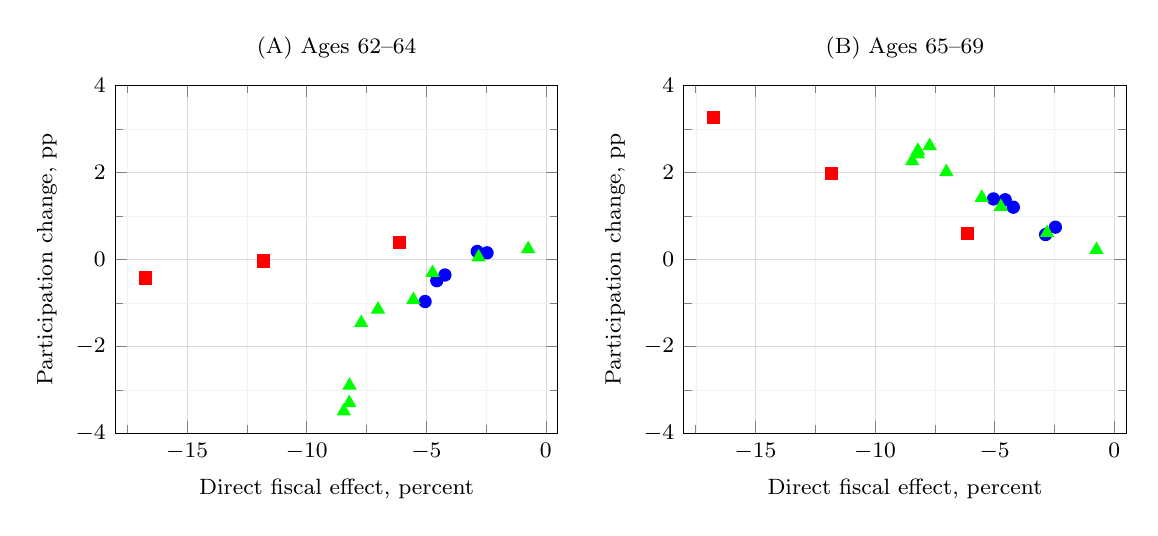
\begin{tikzpicture}
\begin{axis}[%
name=panelA,
width=7.2cm,
height=6cm,
title={(A) Ages 62--64},
title style={font=\footnotesize},
xlabel={Direct fiscal effect, percent},
ylabel={Participation change, pp},
xmin=-18, xmax=0.5,
ymin=-4, ymax=4,
grid=both,
grid style={line width=0.2pt, draw=gray!30},
minor grid style={line width=0.1pt, draw=gray!10},
minor tick num=1,
axis background/.style={fill=white},
tick label style={font=\footnotesize},
label style={font=\footnotesize},
legend to name=legpartsave,
legend columns=3,
legend style={draw=white!15!black, font=\scriptsize, /tikz/every even column/.append style={column sep=0.6em}},
legend cell align=left
]
\addplot [only marks, color=red, mark=square*, mark size=2.2pt] coordinates {(-6.13,0.38) (-11.82,-0.04) (-16.75,-0.43)};          % src: tables/welfare_age_dependence_mvpfv5.tex:108-110
\addlegendentry{Higher NRA (AN1--AN3)}
\addplot [only marks, color=blue, mark=*, mark size=2.2pt] coordinates {(-2.46,0.15) (-2.87,0.18) (-4.22,-0.36) (-4.56,-0.49) (-5.05,-0.97)};   % src: tables/welfare_age_dependence_mvpfv5.tex:112-116
\addlegendentry{Higher DRC (AD1--AD5)}
\addplot [only marks, color=green, mark=triangle*, mark size=2.6pt] coordinates {(-0.74,0.24) (-2.81,0.05) (-4.74,-0.31) (-5.54,-0.93) (-7.02,-1.15) (-7.72,-1.46) (-8.21,-2.90) (-8.22,-3.30) (-8.45,-3.49)};   % src: tables/welfare_age_dependence_mvpfv5.tex:118-126
\addlegendentry{Symmetric adjustment (AL1--AL9)}
\end{axis}
\begin{axis}[%
at={(panelA.east)}, anchor=west, xshift=1.6cm,
width=7.2cm,
height=6cm,
title={(B) Ages 65--69},
title style={font=\footnotesize},
xlabel={Direct fiscal effect, percent},
ylabel={Participation change, pp},
xmin=-18, xmax=0.5,
ymin=-4, ymax=4,
grid=both,
grid style={line width=0.2pt, draw=gray!30},
minor grid style={line width=0.1pt, draw=gray!10},
minor tick num=1,
axis background/.style={fill=white},
tick label style={font=\footnotesize},
label style={font=\footnotesize}
]
\addplot [only marks, color=red, mark=square*, mark size=2.2pt] coordinates {(-6.13,0.60) (-11.82,1.98) (-16.75,3.27)};          % src: tables/welfare_age_dependence_mvpfv5.tex:108-110
\addplot [only marks, color=blue, mark=*, mark size=2.2pt] coordinates {(-2.46,0.74) (-2.87,0.57) (-4.22,1.20) (-4.56,1.37) (-5.05,1.39)};   % src: tables/welfare_age_dependence_mvpfv5.tex:112-116
\addplot [only marks, color=green, mark=triangle*, mark size=2.6pt] coordinates {(-0.74,0.22) (-2.81,0.61) (-4.74,1.21) (-5.54,1.42) (-7.02,2.01) (-7.72,2.61) (-8.21,2.50) (-8.22,2.42) (-8.45,2.26)};   % src: tables/welfare_age_dependence_mvpfv5.tex:118-126
\end{axis}
\end{tikzpicture}

\vspace{2pt}
\pgfplotslegendfromname{legpartsave}

\begin{minipage}{0.92\textwidth}
\vspace{4pt}
\scriptsize
\textit{Notes:} Each marker is one row of \autoref{tab:claiming}. The horizontal axis is the Direct column, the change in the net present value of retirement benefits paid to the cohort as a percentage of its baseline value; the vertical axis is the change in labor force participation in percentage points (pp) at ages 62--64 (panel A) and 65--69 (panel B). Squares: a higher normal retirement age (AN1--AN3); circles: a higher delayed retirement credit (AD1--AD5); triangles: equal early-claiming reductions and delayed credits of $\pm7$ to $\pm15$ percent per year (AL1--AL9). Source: authors' simulations of the estimated model.
% src: tables/welfare_age_dependence_mvpfv5.tex:108-126
\end{minipage}
\end{figure}

\subsection{Participation under the elimination experiments}\label{app:elimlfp}

\autoref{fig:elimlfp} plots labor force participation by age in the estimated model and under the five elimination experiments of \autoref{sec:elimination}, and \autoref{fig:elimlfp_health} repeats the comparison by health state. These figures are the only exhibit of the participation responses to D1--D5; \autoref{tab:elim} reports welfare only. Removing Social Security benefits (D1) raises participation from age 63 by more than any other experiment; removing disability benefits (D5) raises it from age 50, by more than D1 at every age from 50 to 62 except age 60, where the two are within half a percentage point, and most of all among individuals with a disability, the group eligible for the benefit. Full coverage of medical spending after 65 (D2), the full saving subsidy (D3), and removal of the income tax (D4) lower participation at the older ages, D4 by less than the other two from the early 60s.
% src: figures/abdou/frot_weld1_paper.tex and frot_weld2.tex, embedded series rows 50-69 (D5 > D1 at 50-59, 61, 62; D1 > D5 at 60 by 0.34 pp; D1 largest from 63; D4 decline smaller than D2 and D3 from 61); frot_weld1_2_paper.tex, frot_weld2_2.tex (disability panel); no numeric value printed

\begin{figure}[!tp]
\centering
\caption{Labor Force Participation by Age under the Elimination Experiments}
\label{fig:elimlfp}
\vspace{6pt}
\begin{tabular}{cc}
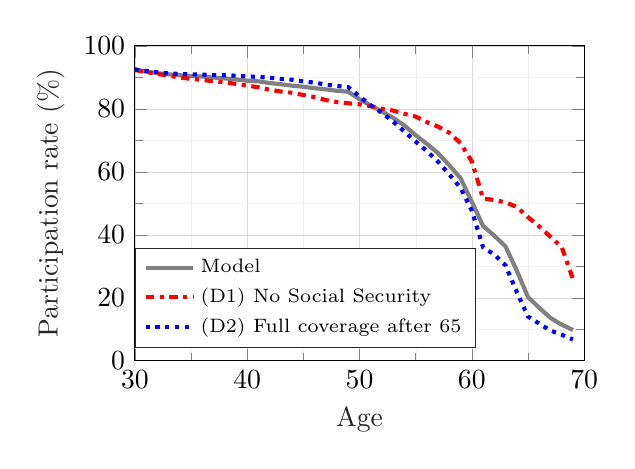
\begin{tikzpicture}
\begin{axis}[%
width=5.706cm,
height=4cm,
at={(0cm,0cm)},
scale only axis,
xmin=30,
xmax=70,
xlabel style={font=\color{white!15!black}},
xlabel={Age},
ymin=-0,
ymax=0100,
ylabel style={font=\color{white!15!black}},
ylabel={Participation rate (\%)},
axis background/.style={fill=white},
%title style={font=\bfseries},
title={},
legend style={at={(axis cs:30,20)}, anchor=west, legend cell align=left, align=left, draw=white!15!black, font=\scriptsize},
grid=both,
grid style={line width=0.2pt, draw=gray!30},
minor grid style={line width=0.1pt, draw=gray!10},
minor tick num=1
]
% Back line (Overall) - full
\addplot [color=gray, line width=1.5pt]
  table[row sep=crcr]{%
30		92.457143	\\
31		91.828571	\\
32		91.314286	\\
33		90.942857	\\
34		90.657143	\\
35		90.4	\\
36		90.257143	\\
37		89.914286	\\
38		89.657143	\\
39		89.314286	\\
40		88.914286	\\
41		88.714286	\\
42		88.171429	\\
43		87.8	\\
44		87.342857	\\
45		87	\\
46		86.542857	\\
47		86.171429	\\
48		85.714286	\\
49		85.428571	\\
50		83.028571	\\
51		81.057143	\\
52		79.142857	\\
53		77.114286	\\
54		74.685714	\\
55		71.628571	\\
56		68.857143	\\
57		65.885714	\\
58		62.028571	\\
59		57.971429	\\
60		50.485714	\\
61		42.771429	\\
62		39.714286	\\
63		36.285714	\\
64		28.657143	\\
65		20.228571	\\
66		16.828571	\\
67		13.6	\\
68		11.457143	\\
69		9.771429	\\
};
\addlegendentry{Model}
% Blue line (Good health) - dotted
\addplot [color=red, line width=1.5pt, dashdotted]
  table[row sep=crcr]{%
30	92.342857	\\
31	91.685714	\\
32	91.057143	\\
33	90.571429	\\
34	89.914286	\\
35	89.514286	\\
36	89.171429	\\
37	88.742857	\\
38	88.371429	\\
39	87.914286	\\
40	87.342857	\\
41	86.857143	\\
42	86.057143	\\
43	85.485714	\\
44	85.085714	\\
45	84.371429	\\
46	83.714286	\\
47	82.771429	\\
48	82.142857	\\
49	81.742857	\\
50	81.428571	\\
51	80.857143	\\
52	79.971429	\\
53	79.428571	\\
54	78.4	\\
55	77.542857	\\
56	75.742857	\\
57	74.314286	\\
58	72.4	\\
59	69.057143	\\
60	63.285714	\\
61	51.542857	\\
62	51.028571	\\
63	50.285714	\\
64	48.857143	\\
65	45.6	\\
66	42.657143	\\
67	39.342857	\\
68	36.114286	\\
69	25.971429	\\
};
\addlegendentry{(D1) No Social Security}

% Red line (Poor health) - dash-dotted
\addplot [color=blue, line width=1.5pt, dotted]
  table[row sep=crcr]{%
30	92.485714	\\
31	92.028571	\\
32	91.6	\\
33	91.228571	\\
34	91.057143	\\
35	90.942857	\\
36	90.857143	\\
37	90.685714	\\
38	90.628571	\\
39	90.514286	\\
40	90.285714	\\
41	90.142857	\\
42	89.885714	\\
43	89.485714	\\
44	89.228571	\\
45	88.685714	\\
46	88.314286	\\
47	87.685714	\\
48	87.257143	\\
49	86.857143	\\
50	83.942857	\\
51	81.085714	\\
52	78.714286	\\
53	75.914286	\\
54	72.742857	\\
55	69.6	\\
56	66.542857	\\
57	63.2	\\
58	59.171429	\\
59	54.857143	\\
60	47.685714	\\
61	36.057143	\\
62	33.714286	\\
63	30.314286	\\
64	21.857143	\\
65	14.057143	\\
66	11.8	\\
67	9.571429	\\
68	8.285714	\\
69	6.742857	\\
};
\addlegendentry{(D2) Full coverage after 65}

% Green line (Disabled) - dashed
% \addplot [color=green, line width=1.5pt, dashed]
%   table[row sep=crcr]{%
% 30	92.6	\\
% 31	92.2	\\
% 32	91.7714286	\\
% 33	91.4285714	\\
% 34	91.2571429	\\
% 35	91.1142857	\\
% 36	91.0571429	\\
% 37	90.8857143	\\
% 38	90.8285714	\\
% 39	90.7142857	\\
% 40	90.4571429	\\
% 41	90.2857143	\\
% 42	90.0285714	\\
% 43	89.6571429	\\
% 44	89.3142857	\\
% 45	88.7714286	\\
% 46	88.2857143	\\
% 47	87.6571429	\\
% 48	87.1714286	\\
% 49	86.6285714	\\
% 50	83.7142857	\\
% 51	80.8285714	\\
% 52	78.5428571	\\
% 53	75.9142857	\\
% 54	72.8857143	\\
% 55	69.7428571	\\
% 56	66.6285714	\\
% 57	63.1428571	\\
% 58	59.0857143	\\
% 59	54.7714286	\\
% 60	47.2571429	\\
% 61	35.0571429	\\
% 62	32.8285714	\\
% 63	29.5714286	\\
% 64	21.0571429	\\
% 65	5.5714286	\\
% 66	3.1428571	\\
% 67	2.0285714	\\
% 68	1.3428571	\\
% 69	0.7142857	\\
% };
% \addlegendentry{Medicare B Reform Full}
\end{axis}
\end{tikzpicture} & 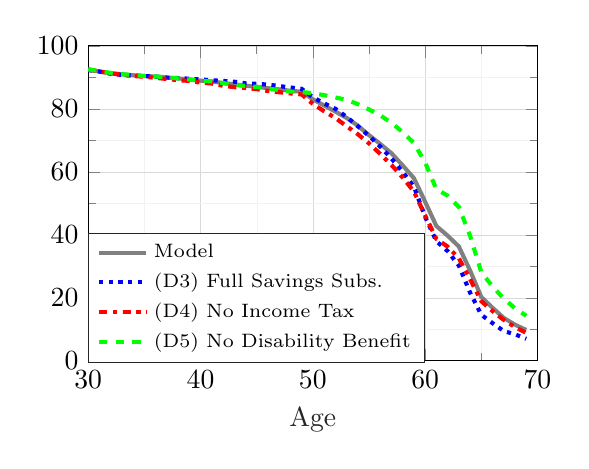
\begin{tikzpicture}
\begin{axis}[%
width=5.706cm,
height=4cm,
at={(0cm,0cm)},
scale only axis,
xmin=30,
xmax=70,
xlabel style={font=\color{white!15!black}},
xlabel={Age},
ymin=-0,
ymax=0100,
ylabel style={font=\color{white!15!black}},
ylabel={},
axis background/.style={fill=white},
%title style={font=\bfseries},
title={},
legend style={at={(axis cs:30,20)}, anchor=west, legend cell align=left, align=left, draw=white!15!black, font=\scriptsize},
grid=both,
grid style={line width=0.2pt, draw=gray!30},
minor grid style={line width=0.1pt, draw=gray!10},
minor tick num=1
]
% Back line (Overall) - full
\addplot [color=gray, line width=1.5pt]
  table[row sep=crcr]{%
30		92.457143	\\
31		91.828571	\\
32		91.314286	\\
33		90.942857	\\
34		90.657143	\\
35		90.4	\\
36		90.257143	\\
37		89.914286	\\
38		89.657143	\\
39		89.314286	\\
40		88.914286	\\
41		88.714286	\\
42		88.171429	\\
43		87.8	\\
44		87.342857	\\
45		87	\\
46		86.542857	\\
47		86.171429	\\
48		85.714286	\\
49		85.428571	\\
50		83.028571	\\
51		81.057143	\\
52		79.142857	\\
53		77.114286	\\
54		74.685714	\\
55		71.628571	\\
56		68.857143	\\
57		65.885714	\\
58		62.028571	\\
59		57.971429	\\
60		50.485714	\\
61		42.771429	\\
62		39.714286	\\
63		36.285714	\\
64		28.657143	\\
65		20.228571	\\
66		16.828571	\\
67		13.6	\\
68		11.457143	\\
69		9.771429	\\
};
\addlegendentry{Model}


% Red line (Poor health) - dash-dotted
\addplot [color=blue, line width=1.5pt, dotted]
  table[row sep=crcr]{%
30	92.285714	\\
31	91.828571	\\
32	91.142857	\\
33	90.742857	\\
34	90.542857	\\
35	90.4	\\
36	90.2	\\
37	89.914286	\\
38	89.742857	\\
39	89.542857	\\
40	89.314286	\\
41	89.057143	\\
42	88.857143	\\
43	88.6	\\
44	88.085714	\\
45	87.914286	\\
46	87.685714	\\
47	87.228571	\\
48	86.771429	\\
49	86.342857	\\
50	83.657143	\\
51	81.742857	\\
52	80.028571	\\
53	77.457143	\\
54	74.485714	\\
55	71.4	\\
56	68	\\
57	64.228571	\\
58	59.942857	\\
59	55.285714	\\
60	45.657143	\\
61	37.971429	\\
62	34.828571	\\
63	30.228571	\\
64	21.657143	\\
65	14.6	\\
66	11.942857	\\
67	9.428571	\\
68	8.4	\\
69	6.971429	\\
};
\addlegendentry{(D3) Full Savings Subs.}
% Blue line (Good health) - dotted
\addplot [color=red, line width=1.5pt, dashdotted]
  table[row sep=crcr]{%
30	92.485714	\\
31	91.857143	\\
32	91.257143	\\
33	90.857143	\\
34	90.428571	\\
35	90.171429	\\
36	89.857143	\\
37	89.457143	\\
38	89.085714	\\
39	88.857143	\\
40	88.314286	\\
41	88.028571	\\
42	87.314286	\\
43	86.885714	\\
44	86.6	\\
45	86.257143	\\
46	85.657143	\\
47	85.257143	\\
48	84.885714	\\
49	84.571429	\\
50	81.571429	\\
51	79.228571	\\
52	77.114286	\\
53	74.485714	\\
54	71.942857	\\
55	69.028571	\\
56	65.685714	\\
57	62.171429	\\
58	58.171429	\\
59	53.714286	\\
60	46.114286	\\
61	38.685714	\\
62	36.257143	\\
63	32.514286	\\
64	25.885714	\\
65	18.914286	\\
66	15.771429	\\
67	12.971429	\\
68	10.685714	\\
69	8.857143	\\
};
\addlegendentry{(D4) No Income Tax}


% Green line (Disabled) - dashed
\addplot [color=green, line width=1.5pt, dashed]
  table[row sep=crcr]{%
30	92.542857	\\
31	91.914286	\\
32	91.4	\\
33	90.971429	\\
34	90.742857	\\
35	90.4	\\
36	90.257143	\\
37	89.942857	\\
38	89.657143	\\
39	89.314286	\\
40	88.942857	\\
41	88.685714	\\
42	88.171429	\\
43	87.6	\\
44	87.257143	\\
45	86.942857	\\
46	86.371429	\\
47	85.971429	\\
48	85.485714	\\
49	85.342857	\\
50	84.942857	\\
51	84.342857	\\
52	83.6	\\
53	82.857143	\\
54	81.485714	\\
55	79.8	\\
56	77.914286	\\
57	75.542857	\\
58	72.571429	\\
59	69.142857	\\
60	62.942857	\\
61	54.428571	\\
62	52.457143	\\
63	48.828571	\\
64	39.685714	\\
65	28.114286	\\
66	23.6	\\
67	19.742857	\\
68	16.685714	\\
69	14.285714	\\
};
\addlegendentry{(D5) No Disability Benefit}
\end{axis}
\end{tikzpicture}
\end{tabular}
\begin{minipage}{0.95\textwidth}\footnotesize\setstretch{1.0}
\textit{Notes:} Labor force participation rate in percent by age, 30--69, in the estimated model (gray) and in the elimination experiments of \autoref{tab:elim}. D1 sets Social Security retirement benefits to zero; D2 sets out-of-pocket medical spending after age 65 to zero for participants and nonparticipants; D3 sets the net return on assets equal to the gross return (the K3 reform of \autoref{tab:other}); D4 sets the income tax to zero; D5 sets disability benefits to zero. Left panel: D1 and D2; right panel: D3--D5. Source: simulations of the estimated model.
% src: 12:325-328 (May 2025 figure notes, rewritten); T:welfare_decomposition_gradient.tex:27-37 (D1-D5 definitions); 5:390 (r -> r_f)
\end{minipage}
\end{figure}

\begin{figure}[!p]
\centering
\caption{Labor Force Participation by Age and Health under the Elimination Experiments}
\label{fig:elimlfp_health}
\vspace{6pt}
\begin{tabular}{cc}
\multicolumn{2}{l}{\footnotesize (A) Good health}\\
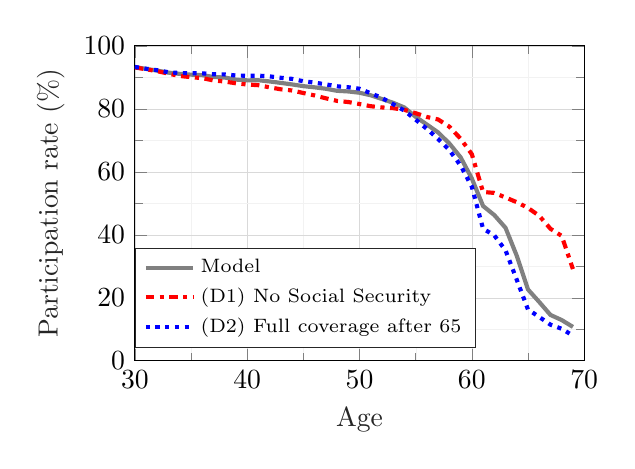
\begin{tikzpicture}
\begin{axis}[%
width=5.706cm,
height=4cm,
at={(0cm,0cm)},
scale only axis,
xmin=30,
xmax=70,
xlabel style={font=\color{white!15!black}},
xlabel={Age},
ymin=-0,
ymax=0100,
ylabel style={font=\color{white!15!black}},
ylabel={Participation rate (\%)},
axis background/.style={fill=white},
%title style={font=\bfseries},
title={},
legend style={at={(axis cs:30,20)}, anchor=west, legend cell align=left, align=left, draw=white!15!black, font=\scriptsize},
grid=both,
grid style={line width=0.2pt, draw=gray!30},
minor grid style={line width=0.1pt, draw=gray!10},
minor tick num=1
]
% Back line (Overall) - full
\addplot [color=gray, line width=1.5pt]
  table[row sep=crcr]{%
30	93.248945	\\
31	92.66386	\\
32	92.127404	\\
33	91.477788	\\
34	91.08492	\\
35	90.842714	\\
36	90.681332	\\
37	90.107527	\\
38	89.928947	\\
39	89.275723	\\
40	89.028213	\\
41	89.071383	\\
42	88.68104	\\
43	88.224061	\\
44	87.736151	\\
45	87.191157	\\
46	86.816406	\\
47	86.369637	\\
48	85.709527	\\
49	85.508219	\\
50	85.099111	\\
51	84.293015	\\
52	83.102493	\\
53	81.913775	\\
54	80.404686	\\
55	77.450628	\\
56	75	\\
57	72.50185	\\
58	68.992537	\\
59	64.610144	\\
60	57.880539	\\
61	49.142634	\\
62	46.258503	\\
63	42.21861	\\
64	33.333333	\\
65	22.642293	\\
66	18.667798	\\
67	14.554196	\\
68	12.927257	\\
69	10.749331	\\
};
\addlegendentry{Model}
% Blue line (Good health) - dotted
\addplot [color=red, line width=1.5pt, dashdotted]
  table[row sep=crcr]{%
30	93.128391	\\
31	92.543596	\\
32	91.947115	\\
33	91.145361	\\
34	90.420066	\\
35	90.051719	\\
36	89.734189	\\
37	89.001536	\\
38	88.662342	\\
39	88.094498	\\
40	87.711599	\\
41	87.492104	\\
42	86.810399	\\
43	86.187142	\\
44	85.814922	\\
45	85.013004	\\
46	84.244792	\\
47	83.333333	\\
48	82.511659	\\
49	82.15364	\\
50	81.510595	\\
51	80.817717	\\
52	80.436288	\\
53	80.196285	\\
54	79.659212	\\
55	78.599641	\\
56	77.405248	\\
57	76.609919	\\
58	74.328358	\\
59	70.514762	\\
60	65.587669	\\
61	53.585347	\\
62	53.301321	\\
63	51.848842	\\
64	50.347648	\\
65	48.525135	\\
66	46.033093	\\
67	41.914336	\\
68	39.658195	\\
69	29.125781	\\
};
\addlegendentry{(D1) No Social Security}

% Red line (Poor health) - dash-dotted
\addplot [color=blue, line width=1.5pt, dotted]
  table[row sep=crcr]{%
30	93.279084	\\
31	92.723993	\\
32	92.247596	\\
33	91.59867	\\
34	91.356905	\\
35	91.268634	\\
36	91.261839	\\
37	90.967742	\\
38	90.917516	\\
39	90.581287	\\
40	90.470219	\\
41	90.524321	\\
42	90.298034	\\
43	89.847231	\\
44	89.497278	\\
45	88.751625	\\
46	88.313802	\\
47	87.755776	\\
48	87.141905	\\
49	86.85005	\\
50	86.363636	\\
51	84.940375	\\
52	83.448753	\\
53	81.458114	\\
54	79.410721	\\
55	76.552962	\\
56	73.61516	\\
57	70.429312	\\
58	66.865672	\\
59	61.998486	\\
60	55.260116	\\
61	41.93297	\\
62	39.815926	\\
63	35.067046	\\
64	25.725971	\\
65	16.285833	\\
66	13.915995	\\
67	11.451049	\\
68	10.166521	\\
69	7.983943	\\
};
\addlegendentry{(D2) Full coverage after 65}

% % Green line (Disabled) - dashed
% \addplot [color=green, line width=1.5pt, dashed]
%   table[row sep=crcr]{%
% 30	88.42857143	\\
% 31	88.22857143	\\
% 32	87.85714286	\\
% 33	86.77142857	\\
% 34	86.57142857	\\
% 35	85.88571429	\\
% 36	85.51428571	\\
% 37	84.77142857	\\
% 38	84.25714286	\\
% 39	83.45714286	\\
% 40	82.62857143	\\
% 41	82.02857143	\\
% 42	81.51428571	\\
% 43	80.82857143	\\
% 44	79.97142857	\\
% 45	78.08571429	\\
% 46	77.54285714	\\
% 47	76	\\
% 48	74.71428571	\\
% 49	73.77142857	\\
% 50	72.02857143	\\
% 51	70.97142857	\\
% 52	68.62857143	\\
% 53	66.31428571	\\
% 54	63.85714286	\\
% 55	60.91428571	\\
% 56	57.57142857	\\
% 57	54.2	\\
% 58	51.11428571	\\
% 59	46.62857143	\\
% 60	40.71428571	\\
% 61	29.94285714	\\
% 62	27.68571429	\\
% 63	23.88571429	\\
% 64	17.48571429	\\
% 65	5.314285714	\\
% 66	3	\\
% 67	1.942857143	\\
% 68	1.257142857	\\
% 69	0.685714286	\\
% };
% \addlegendentry{Medicare B Reform Full}
\end{axis}
\end{tikzpicture} & 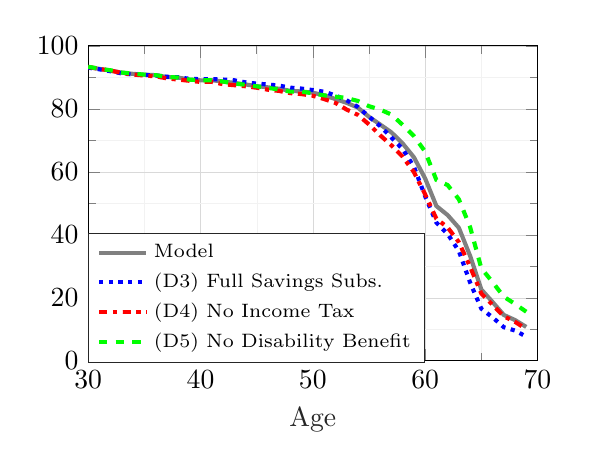
\begin{tikzpicture}
\begin{axis}[%
width=5.706cm,
height=4cm,
at={(0cm,0cm)},
scale only axis,
xmin=30,
xmax=70,
xlabel style={font=\color{white!15!black}},
xlabel={Age},
ymin=-0,
ymax=0100,
ylabel style={font=\color{white!15!black}},
ylabel={},
axis background/.style={fill=white},
%title style={font=\bfseries},
title={},
legend style={at={(axis cs:30,20)}, anchor=west, legend cell align=left, align=left, draw=white!15!black, font=\scriptsize},
grid=both,
grid style={line width=0.2pt, draw=gray!30},
minor grid style={line width=0.1pt, draw=gray!10},
minor tick num=1
]
% Back line (Overall) - full
\addplot [color=gray, line width=1.5pt]
  table[row sep=crcr]{%
30	93.248945	\\
31	92.66386	\\
32	92.127404	\\
33	91.477788	\\
34	91.08492	\\
35	90.842714	\\
36	90.681332	\\
37	90.107527	\\
38	89.928947	\\
39	89.275723	\\
40	89.028213	\\
41	89.071383	\\
42	88.68104	\\
43	88.224061	\\
44	87.736151	\\
45	87.191157	\\
46	86.816406	\\
47	86.369637	\\
48	85.709527	\\
49	85.508219	\\
50	85.099111	\\
51	84.293015	\\
52	83.102493	\\
53	81.913775	\\
54	80.404686	\\
55	77.450628	\\
56	75	\\
57	72.50185	\\
58	68.992537	\\
59	64.610144	\\
60	57.880539	\\
61	49.142634	\\
62	46.258503	\\
63	42.21861	\\
64	33.333333	\\
65	22.642293	\\
66	18.667798	\\
67	14.554196	\\
68	12.927257	\\
69	10.749331	\\
};
\addlegendentry{Model}


% Red line (Poor health) - dash-dotted
\addplot [color=blue, line width=1.5pt, dotted]
  table[row sep=crcr]{%
30	93.068113	\\
31	92.543596	\\
32	91.917067	\\
33	91.205802	\\
34	90.903596	\\
35	90.751445	\\
36	90.55912	\\
37	90.168971	\\
38	90.021625	\\
39	89.524402	\\
40	89.404389	\\
41	89.418825	\\
42	89.28345	\\
43	89.05156	\\
44	88.408581	\\
45	88.003901	\\
46	87.727865	\\
47	87.359736	\\
48	86.708861	\\
49	86.413955	\\
50	85.95352	\\
51	85.417376	\\
52	84.279778	\\
53	82.719944	\\
54	80.617678	\\
55	77.522442	\\
56	74.489796	\\
57	70.873427	\\
58	67.201493	\\
59	61.619985	\\
60	52.2158	\\
61	43.842557	\\
62	40.256102	\\
63	34.863876	\\
64	24.867076	\\
65	16.535106	\\
66	13.788714	\\
67	10.664336	\\
68	9.596845	\\
69	7.671722	\\
};
\addlegendentry{(D3) Full Savings Subs.}


% Blue line (Good health) - dotted
\addplot [color=red, line width=1.5pt, dashdotted]
  table[row sep=crcr]{%
30	93.279084	\\
31	92.66386	\\
32	92.097356	\\
33	91.387126	\\
34	90.873376	\\
35	90.568908	\\
36	90.314696	\\
37	89.677419	\\
38	89.280198	\\
39	88.902704	\\
40	88.526646	\\
41	88.566014	\\
42	87.824984	\\
43	87.492043	\\
44	87.159782	\\
45	86.703511	\\
46	86.067708	\\
47	85.676568	\\
48	84.976682	\\
49	84.669574	\\
50	84.142174	\\
51	83.100511	\\
52	81.890582	\\
53	79.775675	\\
54	78.097267	\\
55	75.044883	\\
56	71.574344	\\
57	68.393782	\\
58	64.776119	\\
59	59.91673	\\
60	52.83237	\\
61	45.089634	\\
62	42.336935	\\
63	37.667615	\\
64	29.856851	\\
65	21.354383	\\
66	17.776835	\\
67	14.117133	\\
68	12.357581	\\
69	10.080285	\\
};
\addlegendentry{(D4) No Income Tax}
% Green line (Disabled) - dashed
\addplot [color=green, line width=1.5pt, dashed]
  table[row sep=crcr]{%
30	93.339361	\\
31	92.723993	\\
32	92.217548	\\
33	91.508008	\\
34	91.175582	\\
35	90.842714	\\
36	90.681332	\\
37	90.138249	\\
38	89.928947	\\
39	89.275723	\\
40	89.059561	\\
41	89.039798	\\
42	88.649334	\\
43	88.0331	\\
44	87.64009	\\
45	87.126138	\\
46	86.653646	\\
47	86.138614	\\
48	85.443038	\\
49	85.441127	\\
50	84.92823	\\
51	84.258944	\\
52	83.864266	\\
53	83.42096	\\
54	82.499113	\\
55	80.825853	\\
56	79.737609	\\
57	78.164323	\\
58	74.88806	\\
59	71.347464	\\
60	66.396917	\\
61	57.404521	\\
62	55.782313	\\
63	51.279967	\\
64	42.494888	\\
65	29.372663	\\
66	24.989393	\\
67	20.323427	\\
68	18.054338	\\
69	15.566459	\\
};
\addlegendentry{(D5) No Disability Benefit}
\end{axis}
\end{tikzpicture}\\
\multicolumn{2}{l}{\footnotesize (B) Poor health}\\
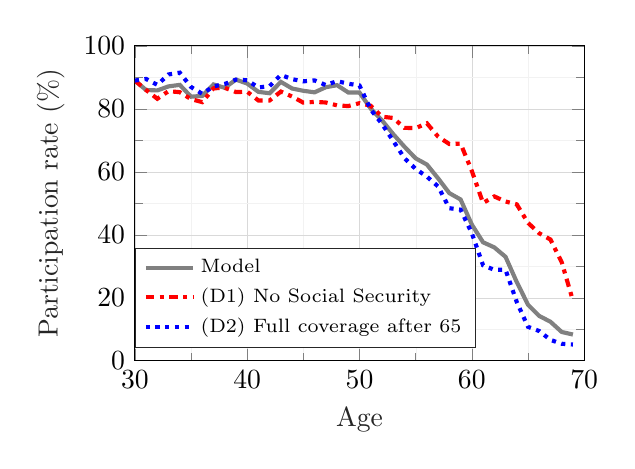
\begin{tikzpicture}
\begin{axis}[%
width=5.706cm,
height=4cm,
at={(0cm,0cm)},
scale only axis,
xmin=30,
xmax=70,
xlabel style={font=\color{white!15!black}},
xlabel={Age},
ymin=-0,
ymax=0100,
ylabel style={font=\color{white!15!black}},
ylabel={Participation rate (\%)},
axis background/.style={fill=white},
%title style={font=\bfseries},
title={},
legend style={at={(axis cs:30,20)}, anchor=west, legend cell align=left, align=left, draw=white!15!black, font=\scriptsize},
grid=both,
grid style={line width=0.2pt, draw=gray!30},
minor grid style={line width=0.1pt, draw=gray!10},
minor tick num=1
]
% Back line (Overall) - full
\addplot [color=gray, line width=1.5pt]
  table[row sep=crcr]{%
30	88.970588	\\
31	85.964912	\\
32	85.840708	\\
33	87.121212	\\
34	87.596899	\\
35	83.846154	\\
36	84.10596	\\
37	87.730061	\\
38	86.666667	\\
39	89.265537	\\
40	88.020833	\\
41	85.388128	\\
42	84.931507	\\
43	88.546256	\\
44	86.440678	\\
45	85.714286	\\
46	85.227273	\\
47	86.851211	\\
48	87.5	\\
49	85.185185	\\
50	85.154062	\\
51	80.060423	\\
52	76.353276	\\
53	71.967655	\\
54	67.96875	\\
55	64.268585	\\
56	62.302483	\\
57	57.905983	\\
58	53.222453	\\
59	51.209677	\\
60	43.248532	\\
61	37.619962	\\
62	36	\\
63	33.004926	\\
64	25	\\
65	17.810458	\\
66	14.24	\\
67	12.389381	\\
68	9.145427	\\
69	8.333333	\\
};
\addlegendentry{Model}
% Blue line (Good health) - dotted
\addplot [color=red, line width=1.5pt, dashdotted]
  table[row sep=crcr]{%
30	88.970588	\\
31	85.964912	\\
32	83.185841	\\
33	85.606061	\\
34	85.271318	\\
35	83.076923	\\
36	82.119205	\\
37	86.503067	\\
38	86.666667	\\
39	85.310734	\\
40	85.416667	\\
41	82.648402	\\
42	82.648402	\\
43	85.462555	\\
44	83.898305	\\
45	81.954887	\\
46	82.19697	\\
47	82.00692	\\
48	81.089744	\\
49	80.864198	\\
50	81.792717	\\
51	80.966767	\\
52	77.492877	\\
53	77.088949	\\
54	73.958333	\\
55	73.860911	\\
56	75.395034	\\
57	71.153846	\\
58	68.814969	\\
59	68.951613	\\
60	60.273973	\\
61	50.095969	\\
62	52.173913	\\
63	50.574713	\\
64	49.666667	\\
65	43.79085	\\
66	40.48	\\
67	38.495575	\\
68	31.334333	\\
69	19.109195	\\
};
\addlegendentry{(D1) No Social Security}

% Red line (Poor health) - dash-dotted
\addplot [color=blue, line width=1.5pt, dotted]
  table[row sep=crcr]{%
30	88.970588	\\
31	89.473684	\\
32	87.610619	\\
33	90.909091	\\
34	91.472868	\\
35	86.923077	\\
36	84.768212	\\
37	87.116564	\\
38	87.878788	\\
39	89.265537	\\
40	89.0625	\\
41	86.757991	\\
42	87.214612	\\
43	90.748899	\\
44	89.40678	\\
45	88.721805	\\
46	89.015152	\\
47	87.543253	\\
48	88.782051	\\
49	87.962963	\\
50	87.394958	\\
51	79.758308	\\
52	75.213675	\\
53	69.811321	\\
54	64.322917	\\
55	60.911271	\\
56	58.465011	\\
57	55.34188	\\
58	48.440748	\\
59	47.983871	\\
60	40.508806	\\
61	30.326296	\\
62	28.869565	\\
63	28.899836	\\
64	18.666667	\\
65	10.784314	\\
66	9.44	\\
67	6.637168	\\
68	5.397301	\\
69	5.172414	\\
};
\addlegendentry{(D2) Full coverage after 65}

% % Green line (Disabled) - dashed
% \addplot [color=green, line width=1.5pt, dashed]
%   table[row sep=crcr]{%
% 30	91.91176471	\\
% 31	89.47368421	\\
% 32	88.49557522	\\
% 33	91.66666667	\\
% 34	91.47286822	\\
% 35	86.92307692	\\
% 36	85.43046358	\\
% 37	87.73006135	\\
% 38	88.48484848	\\
% 39	89.26553672	\\
% 40	89.0625	\\
% 41	86.75799087	\\
% 42	87.21461187	\\
% 43	90.74889868	\\
% 44	88.98305085	\\
% 45	88.72180451	\\
% 46	88.63636364	\\
% 47	87.5432526	\\
% 48	88.46153846	\\
% 49	87.34567901	\\
% 50	86.55462185	\\
% 51	79.15407855	\\
% 52	76.06837607	\\
% 53	70.08086253	\\
% 54	64.32291667	\\
% 55	60.19184652	\\
% 56	59.36794582	\\
% 57	55.55555556	\\
% 58	48.23284823	\\
% 59	47.58064516	\\
% 60	38.94324853	\\
% 61	28.59884837	\\
% 62	28	\\
% 63	28.40722496	\\
% 64	17.16666667	\\
% 65	0.653594771	\\
% 66	0.64	\\
% 67	0.147492625	\\
% 68	0.149925037	\\
% 69	0	\\
% };
% \addlegendentry{Medicare B Reform Full}
\end{axis}
\end{tikzpicture} & 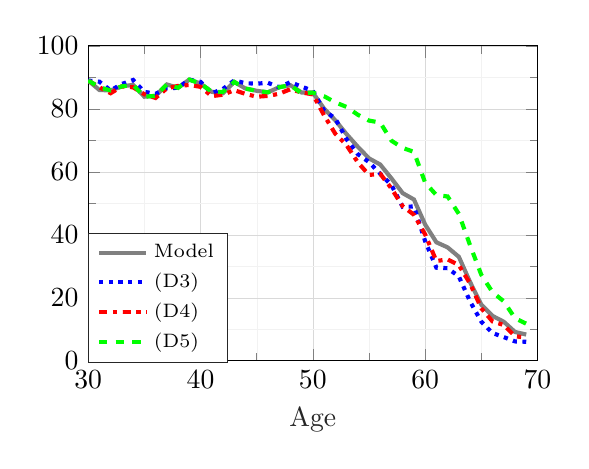
\begin{tikzpicture}
\begin{axis}[%
width=5.706cm,
height=4cm,
at={(0cm,0cm)},
scale only axis,
xmin=30,
xmax=70,
xlabel style={font=\color{white!15!black}},
xlabel={Age},
ymin=-0,
ymax=0100,
ylabel style={font=\color{white!15!black}},
ylabel={},
axis background/.style={fill=white},
%title style={font=\bfseries},
title={},
legend style={at={(axis cs:30,20)}, anchor=west, legend cell align=left, align=left, draw=white!15!black, font=\scriptsize},
grid=both,
grid style={line width=0.2pt, draw=gray!30},
minor grid style={line width=0.1pt, draw=gray!10},
minor tick num=1
]
% Back line (Overall) - full
\addplot [color=gray, line width=1.5pt]
  table[row sep=crcr]{%
30	88.970588	\\
31	85.964912	\\
32	85.840708	\\
33	87.121212	\\
34	87.596899	\\
35	83.846154	\\
36	84.10596	\\
37	87.730061	\\
38	86.666667	\\
39	89.265537	\\
40	88.020833	\\
41	85.388128	\\
42	84.931507	\\
43	88.546256	\\
44	86.440678	\\
45	85.714286	\\
46	85.227273	\\
47	86.851211	\\
48	87.5	\\
49	85.185185	\\
50	85.154062	\\
51	80.060423	\\
52	76.353276	\\
53	71.967655	\\
54	67.96875	\\
55	64.268585	\\
56	62.302483	\\
57	57.905983	\\
58	53.222453	\\
59	51.209677	\\
60	43.248532	\\
61	37.619962	\\
62	36	\\
63	33.004926	\\
64	25	\\
65	17.810458	\\
66	14.24	\\
67	12.389381	\\
68	9.145427	\\
69	8.333333	\\
};
\addlegendentry{Model}

% Red line (Poor health) - dash-dotted
\addplot [color=blue, line width=1.5pt, dotted]
  table[row sep=crcr]{%
30	88.970588	\\
31	88.596491	\\
32	85.840708	\\
33	87.878788	\\
34	89.147287	\\
35	85.384615	\\
36	84.768212	\\
37	86.503067	\\
38	86.666667	\\
39	89.265537	\\
40	88.541667	\\
41	84.931507	\\
42	86.30137	\\
43	88.986784	\\
44	88.135593	\\
45	87.969925	\\
46	88.257576	\\
47	86.851211	\\
48	88.461538	\\
49	87.037037	\\
50	85.714286	\\
51	79.456193	\\
52	76.923077	\\
53	70.350404	\\
54	65.625	\\
55	63.069544	\\
56	59.367946	\\
57	55.769231	\\
58	48.856549	\\
59	48.991935	\\
60	37.964775	\\
61	29.558541	\\
62	29.391304	\\
63	26.765189	\\
64	18.833333	\\
65	12.418301	\\
66	8.8	\\
67	7.522124	\\
68	6.146927	\\
69	6.034483	\\
};
%\addlegendentry{(D3) No Cap. Gains Tax}
\addlegendentry{(D3)}
% Blue line (Good health) - dotted
\addplot [color=red, line width=1.5pt, dashdotted]
  table[row sep=crcr]{%
30	88.970588	\\
31	86.842105	\\
32	84.955752	\\
33	87.121212	\\
34	86.821705	\\
35	84.615385	\\
36	83.443709	\\
37	86.503067	\\
38	87.272727	\\
39	87.570621	\\
40	86.979167	\\
41	84.018265	\\
42	84.474886	\\
43	85.903084	\\
44	84.745763	\\
45	83.834586	\\
46	84.090909	\\
47	84.775087	\\
48	86.217949	\\
49	85.185185	\\
50	84.593838	\\
51	77.945619	\\
52	72.079772	\\
53	68.463612	\\
54	63.020833	\\
55	58.992806	\\
56	59.367946	\\
57	54.700855	\\
58	49.064449	\\
59	46.370968	\\
60	40.117417	\\
61	31.669866	\\
62	32.173913	\\
63	30.377668	\\
64	24.5	\\
65	16.666667	\\
66	12.48	\\
67	11.356932	\\
68	7.796102	\\
69	7.327586	\\
};
%\addlegendentry{(D4) No Income Tax}
\addlegendentry{(D4)}



% Green line (Disabled) - dashed
\addplot [color=green, line width=1.5pt, dashed]
  table[row sep=crcr]{%
30	88.970588	\\
31	86.842105	\\
32	85.840708	\\
33	87.121212	\\
34	87.596899	\\
35	83.846154	\\
36	84.10596	\\
37	87.730061	\\
38	86.666667	\\
39	89.265537	\\
40	88.020833	\\
41	85.388128	\\
42	85.388128	\\
43	88.546256	\\
44	86.440678	\\
45	85.714286	\\
46	85.227273	\\
47	86.851211	\\
48	87.5	\\
49	84.876543	\\
50	85.154062	\\
51	83.987915	\\
52	82.051282	\\
53	80.592992	\\
54	78.125	\\
55	76.258993	\\
56	75.620767	\\
57	69.871795	\\
58	67.567568	\\
59	66.330645	\\
60	56.555773	\\
61	52.591171	\\
62	52.173913	\\
63	46.633826	\\
64	36.666667	\\
65	27.287582	\\
66	21.76	\\
67	18.879056	\\
68	13.493253	\\
69	11.781609	\\
};
%\addlegendentry{(D5) No Disability Benefit}
\addlegendentry{(D5)}
\end{axis}
\end{tikzpicture}\\
\multicolumn{2}{l}{\footnotesize (C) With a disability}\\
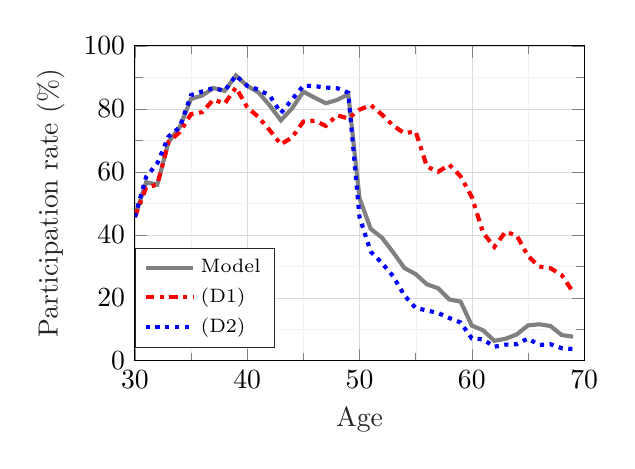
\begin{tikzpicture}
\begin{axis}[%
width=5.706cm,
height=4cm,
at={(0cm,0cm)},
scale only axis,
xmin=30,
xmax=70,
xlabel style={font=\color{white!15!black}},
xlabel={Age},
ymin=-0,
ymax=0100,
ylabel style={font=\color{white!15!black}},
ylabel={Participation rate (\%)},
axis background/.style={fill=white},
%title style={font=\bfseries},
title={},
legend style={at={(axis cs:30,20)}, anchor=west, legend cell align=left, align=left, draw=white!15!black, font=\scriptsize},
grid=both,
grid style={line width=0.2pt, draw=gray!30},
minor grid style={line width=0.1pt, draw=gray!10},
minor tick num=1
]
% Back line (Overall) - full
\addplot [color=gray, line width=1.5pt]
  table[row sep=crcr]{%
30	45.652174	\\
31	56.666667	\\
32	55.932203	\\
33	69.491525	\\
34	74.193548	\\
35	83.13253	\\
36	84.210526	\\
37	86.585366	\\
38	85.714286	\\
39	90.566038	\\
40	87.288136	\\
41	85.217391	\\
42	81.102362	\\
43	76.335878	\\
44	80.141844	\\
45	85.443038	\\
46	83.536585	\\
47	81.767956	\\
48	82.795699	\\
49	84.615385	\\
50	51.612903	\\
51	41.880342	\\
52	39.08046	\\
53	34.42029	\\
54	29.431438	\\
55	27.516779	\\
56	24.28115	\\
57	23.030303	\\
58	19.469027	\\
59	18.78453	\\
60	11.167513	\\
61	9.68523	\\
62	6.338028	\\
63	6.976744	\\
64	8.351648	\\
65	11.226611	\\
66	11.583012	\\
67	11.048689	\\
68	8.166969	\\
69	7.651246	\\
};
\addlegendentry{Model}
% Blue line (Good health) - dotted
\addplot [color=red, line width=1.5pt, dashdotted]
  table[row sep=crcr]{%
30	45.652174	\\
31	55	\\
32	55.932203	\\
33	69.491525	\\
34	72.580645	\\
35	78.313253	\\
36	78.947368	\\
37	82.926829	\\
38	81.632653	\\
39	86.792453	\\
40	80.508475	\\
41	77.391304	\\
42	73.228346	\\
43	68.70229	\\
44	70.921986	\\
45	75.949367	\\
46	76.219512	\\
47	74.585635	\\
48	77.956989	\\
49	76.923077	\\
50	79.723502	\\
51	81.196581	\\
52	78.16092	\\
53	74.637681	\\
54	72.240803	\\
55	72.818792	\\
56	61.661342	\\
57	60	\\
58	62.241888	\\
59	58.563536	\\
60	52.030457	\\
61	40.677966	\\
62	36.150235	\\
63	40.930233	\\
64	39.78022	\\
65	33.264033	\\
66	29.92278	\\
67	29.400749	\\
68	27.22323	\\
69	21.886121	\\
};
%\addlegendentry{(D1) No Social Security}
\addlegendentry{(D1)}

% Red line (Poor health) - dash-dotted
\addplot [color=blue, line width=1.5pt, dotted]
  table[row sep=crcr]{%
30	45.652174	\\
31	58.333333	\\
32	62.711864	\\
33	71.186441	\\
34	74.193548	\\
35	84.337349	\\
36	85.526316	\\
37	86.585366	\\
38	85.714286	\\
39	90.566038	\\
40	87.288136	\\
41	86.086957	\\
42	84.251969	\\
43	78.625954	\\
44	82.978723	\\
45	87.341772	\\
46	87.195122	\\
47	86.740331	\\
48	86.55914	\\
49	85.128205	\\
50	45.62212	\\
51	34.615385	\\
52	31.034483	\\
53	26.811594	\\
54	20.735786	\\
55	16.778523	\\
56	15.974441	\\
57	15.151515	\\
58	13.569322	\\
59	12.154696	\\
60	7.106599	\\
61	6.779661	\\
62	4.460094	\\
63	5.116279	\\
64	5.274725	\\
65	7.068607	\\
66	5.019305	\\
67	5.243446	\\
68	3.99274	\\
69	3.736655	\\
};
%\addlegendentry{(D2) Full coverage after 65}
\addlegendentry{(D2)}

% Green line (Disabled) - dashed
% \addplot [color=green, line width=1.5pt, dashed]
%   table[row sep=crcr]{%
% 30	45.65217391	\\
% 31	61.66666667	\\
% 32	62.71186441	\\
% 33	71.18644068	\\
% 34	74.19354839	\\
% 35	84.3373494	\\
% 36	85.52631579	\\
% 37	86.58536585	\\
% 38	85.71428571	\\
% 39	90.56603774	\\
% 40	87.28813559	\\
% 41	86.08695652	\\
% 42	84.2519685	\\
% 43	78.6259542	\\
% 44	82.9787234	\\
% 45	87.34177215	\\
% 46	86.58536585	\\
% 47	85.63535912	\\
% 48	86.02150538	\\
% 49	85.64102564	\\
% 50	46.08294931	\\
% 51	35.47008547	\\
% 52	30.651341	\\
% 53	27.53623188	\\
% 54	23.07692308	\\
% 55	19.46308725	\\
% 56	17.25239617	\\
% 57	16.06060606	\\
% 58	13.86430678	\\
% 59	13.5359116	\\
% 60	7.614213198	\\
% 61	7.263922518	\\
% 62	4.460093897	\\
% 63	6.046511628	\\
% 64	4.835164835	\\
% 65	1.03950104	\\
% 66	0.193050193	\\
% 67	0.374531835	\\
% 68	0.362976407	\\
% 69	0.177935943	\\
% };
% \addlegendentry{Medicare B Reform Full}
\end{axis}
\end{tikzpicture} & 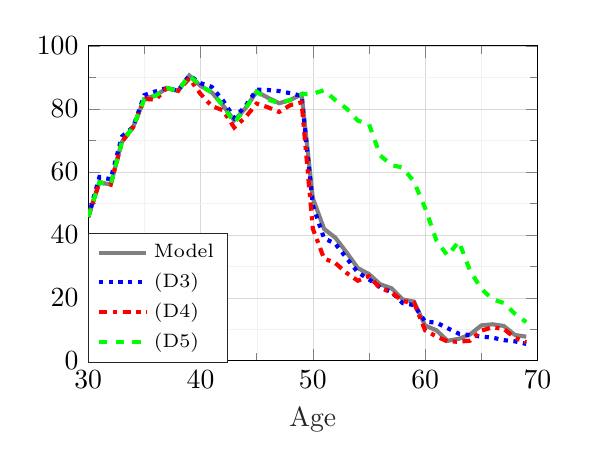
\begin{tikzpicture}
\begin{axis}[%
width=5.706cm,
height=4cm,
at={(0cm,0cm)},
scale only axis,
xmin=30,
xmax=70,
xlabel style={font=\color{white!15!black}},
xlabel={Age},
ymin=-0,
ymax=0100,
ylabel style={font=\color{white!15!black}},
ylabel={},
axis background/.style={fill=white},
%title style={font=\bfseries},
title={},
legend style={at={(axis cs:30,20)}, anchor=west, legend cell align=left, align=left, draw=white!15!black, font=\scriptsize},
grid=both,
grid style={line width=0.2pt, draw=gray!30},
minor grid style={line width=0.1pt, draw=gray!10},
minor tick num=1
]
% Back line (Overall) - full
\addplot [color=gray, line width=1.5pt]
  table[row sep=crcr]{%
30	45.652174	\\
31	56.666667	\\
32	55.932203	\\
33	69.491525	\\
34	74.193548	\\
35	83.13253	\\
36	84.210526	\\
37	86.585366	\\
38	85.714286	\\
39	90.566038	\\
40	87.288136	\\
41	85.217391	\\
42	81.102362	\\
43	76.335878	\\
44	80.141844	\\
45	85.443038	\\
46	83.536585	\\
47	81.767956	\\
48	82.795699	\\
49	84.615385	\\
50	51.612903	\\
51	41.880342	\\
52	39.08046	\\
53	34.42029	\\
54	29.431438	\\
55	27.516779	\\
56	24.28115	\\
57	23.030303	\\
58	19.469027	\\
59	18.78453	\\
60	11.167513	\\
61	9.68523	\\
62	6.338028	\\
63	6.976744	\\
64	8.351648	\\
65	11.226611	\\
66	11.583012	\\
67	11.048689	\\
68	8.166969	\\
69	7.651246	\\
};
\addlegendentry{Model}

% Red line (Poor health) - dash-dotted
\addplot [color=blue, line width=1.5pt, dotted]
  table[row sep=crcr]{%
30	45.652174	\\
31	58.333333	\\
32	57.627119	\\
33	71.186441	\\
34	74.193548	\\
35	84.337349	\\
36	85.526316	\\
37	86.585366	\\
38	85.714286	\\
39	90.566038	\\
40	88.135593	\\
41	86.956522	\\
42	82.677165	\\
43	77.099237	\\
44	80.851064	\\
45	86.075949	\\
46	85.97561	\\
47	85.635359	\\
48	84.946237	\\
49	84.102564	\\
50	49.308756	\\
51	38.888889	\\
52	37.164751	\\
53	32.608696	\\
54	28.093645	\\
55	25.838926	\\
56	23.322684	\\
57	21.818182	\\
58	18.289086	\\
59	17.679558	\\
60	12.436548	\\
61	12.106538	\\
62	10.328638	\\
63	8.604651	\\
64	8.131868	\\
65	7.692308	\\
66	7.335907	\\
67	6.554307	\\
68	6.170599	\\
69	5.338078	\\
};
%\addlegendentry{(D3) No Cap. Gains Tax}
\addlegendentry{(D3)}
% Blue line (Good health) - dotted
\addplot [color=red, line width=1.5pt, dashdotted]
  table[row sep=crcr]{%
30	45.652174	\\
31	56.666667	\\
32	55.932203	\\
33	69.491525	\\
34	74.193548	\\
35	83.13253	\\
36	82.894737	\\
37	86.585366	\\
38	85.714286	\\
39	89.622642	\\
40	84.745763	\\
41	80.869565	\\
42	79.527559	\\
43	74.045802	\\
44	77.304965	\\
45	81.64557	\\
46	80.487805	\\
47	79.005525	\\
48	81.182796	\\
49	82.051282	\\
50	41.935484	\\
51	32.478632	\\
52	31.034483	\\
53	27.898551	\\
54	25.41806	\\
55	26.845638	\\
56	23.003195	\\
57	21.818182	\\
58	18.879056	\\
59	18.508287	\\
60	9.64467	\\
61	7.748184	\\
62	6.103286	\\
63	6.046512	\\
64	6.373626	\\
65	9.56341	\\
66	10.617761	\\
67	10.11236	\\
68	7.259528	\\
69	5.871886	\\
};
%\addlegendentry{(D4) No Income Tax}
\addlegendentry{(D4)}


% Green line (Disabled) - dashed
\addplot [color=green, line width=1.5pt, dashed]
  table[row sep=crcr]{%
30	45.652174	\\
31	56.666667	\\
32	55.932203	\\
33	69.491525	\\
34	74.193548	\\
35	83.13253	\\
36	84.210526	\\
37	86.585366	\\
38	85.714286	\\
39	90.566038	\\
40	87.288136	\\
41	85.217391	\\
42	81.102362	\\
43	75.572519	\\
44	80.141844	\\
45	85.443038	\\
46	82.926829	\\
47	81.767956	\\
48	82.795699	\\
49	84.615385	\\
50	84.792627	\\
51	85.897436	\\
52	82.758621	\\
53	80.072464	\\
54	76.254181	\\
55	75.167785	\\
56	65.175719	\\
57	62.121212	\\
58	61.356932	\\
59	56.906077	\\
60	48.477157	\\
61	38.256659	\\
62	33.333333	\\
63	37.906977	\\
64	28.571429	\\
65	22.869023	\\
66	19.498069	\\
67	18.35206	\\
68	14.882033	\\
69	12.27758	\\
};
%\addlegendentry{(D5) No Disability Benefit}
\addlegendentry{(D5)}
\end{axis}
\end{tikzpicture}
\end{tabular}
\begin{minipage}{0.95\textwidth}\footnotesize\setstretch{1.0}
\textit{Notes:} Labor force participation rate in percent by age, 30--69, by current health state, in the estimated model (gray) and in the elimination experiments of \autoref{tab:elim}: D1 sets Social Security retirement benefits to zero; D2 sets out-of-pocket medical spending after age 65 to zero; D3 sets the net return on assets equal to the gross return; D4 sets the income tax to zero; D5 sets disability benefits to zero. In panels (B) and (C) the legend abbreviates the experiment labels to their identifiers. Source: simulations of the estimated model.
% src: 12:368-374 (May 2025 figure notes, rewritten); figures/abdou/frot_weld1_2.tex:114,161 and frot_weld2_1.tex:115,161,210 (abbreviated legends)
\end{minipage}
\end{figure}

% Final fix pass: the \FloatBarrier that closed Appendix C was removed. It forced Figure C3 (a full-page float) onto its own page and left the preceding page about 40 percent blank; without it the text of Appendix D fills that page and Figure C3 floats onto the page after it.
